\section{Requirements}

\subsection{User Stories}
\begin{comment}
Use the template from the course website and list all user stories here. It is
fine to have them in an spreadsheet (or other applications, such as Trello) at
first, but they must end up here as well.

These user stories should describe what the user will be able to do. Write
the user stories in language of the customer, and give them a unique ID. List
the user stories in order of priority.

You need to annotate an user story whether or not it is implemented. We need to
know which user stories are implemented, such that we can check this during the
oral presentation.
\end{comment}

\subsection{Definition of Done}
\begin{comment}
In this section you list the acceptance criteria that are common for all user
stories. For example, the code should reviewed and tests, it should be under
version control, etc.
\end{comment}

\subsection{User interface}
\begin{comment}
Include sketches, drawings and explanations of the application's user interface.
Describe the navigation between the different views.
\end{comment}
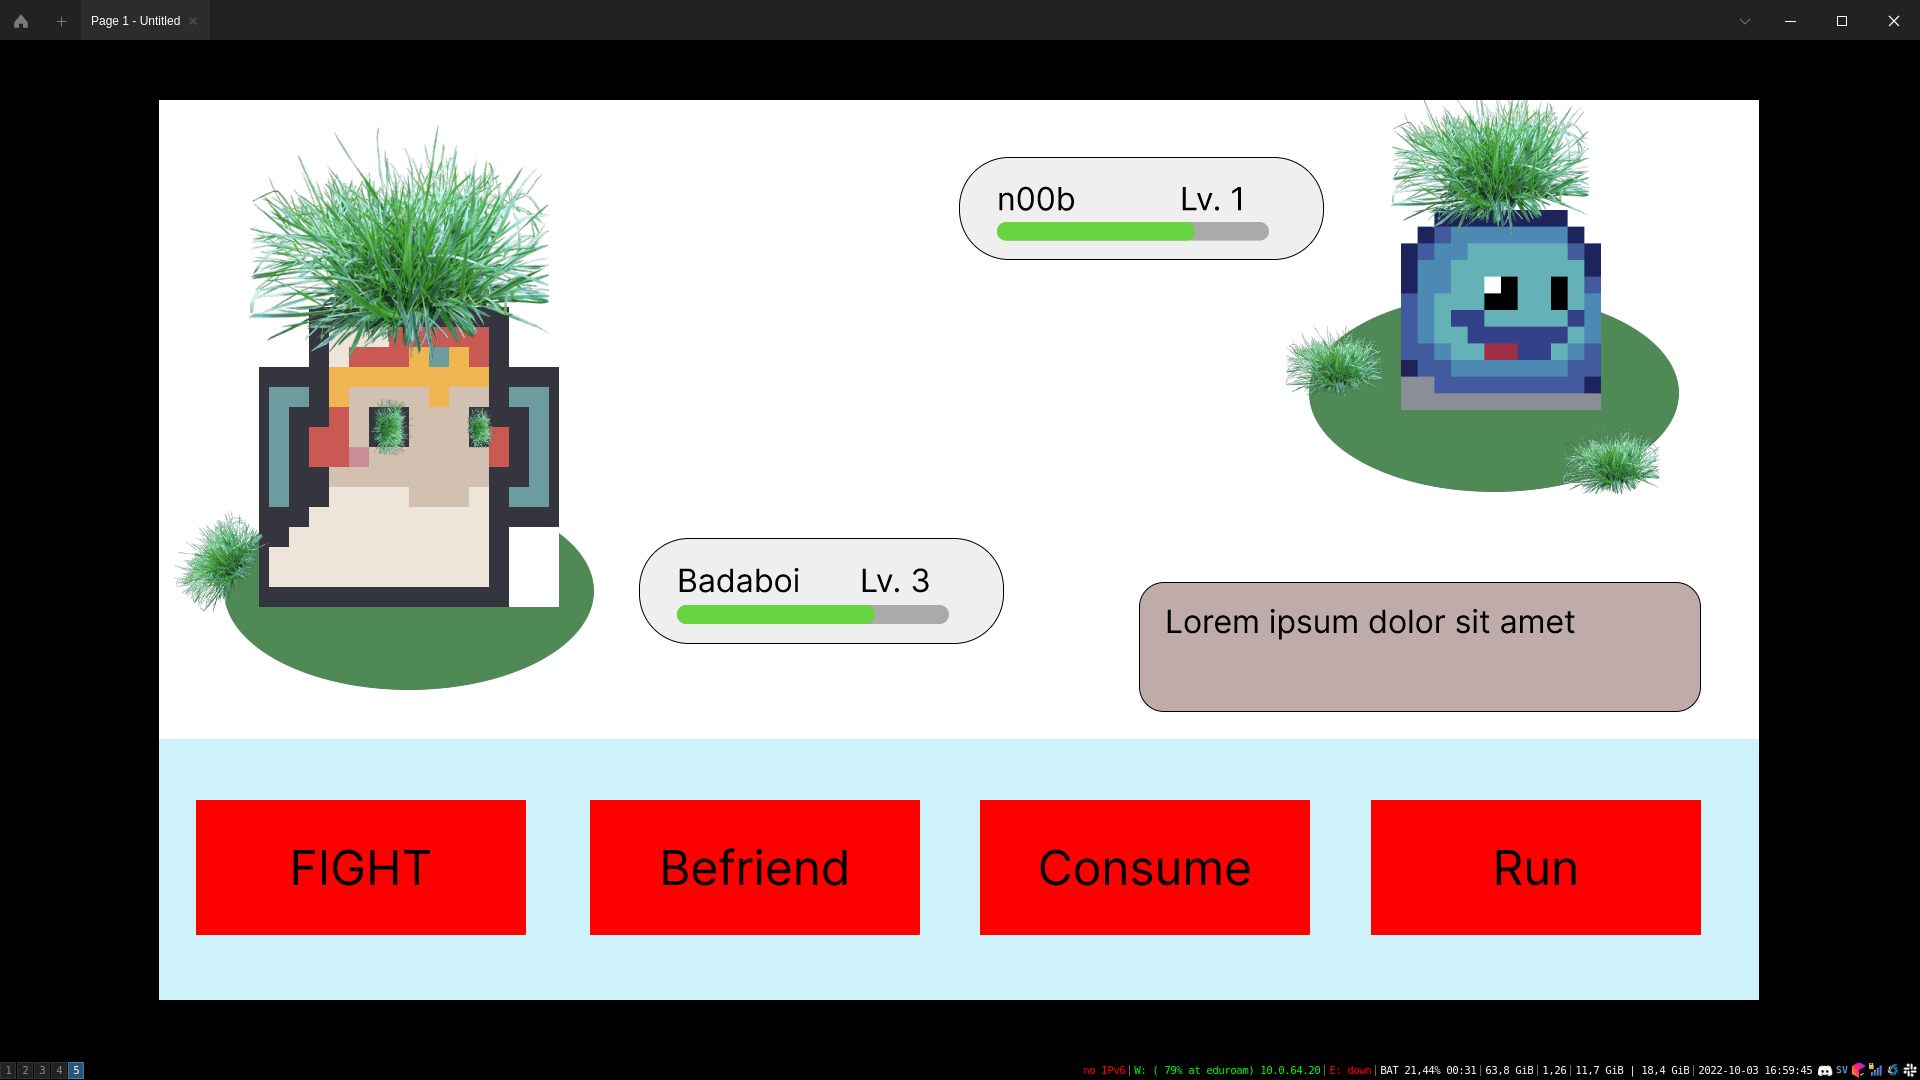
\includegraphics[width=\textwidth]{images/combat_figma.png}